% Options for packages loaded elsewhere
\PassOptionsToPackage{unicode}{hyperref}
\PassOptionsToPackage{hyphens}{url}
\documentclass[
  american,
  11pt,
]{article}
\usepackage{xcolor}
\usepackage[margin=25mm]{geometry}
\usepackage{amsmath,amssymb}
\setcounter{secnumdepth}{-\maxdimen} % remove section numbering
\usepackage{iftex}
\ifPDFTeX
  \usepackage[T1]{fontenc}
  \usepackage[utf8]{inputenc}
  \usepackage{textcomp} % provide euro and other symbols
\else % if luatex or xetex
  \usepackage{unicode-math} % this also loads fontspec
  \defaultfontfeatures{Scale=MatchLowercase}
  \defaultfontfeatures[\rmfamily]{Ligatures=TeX,Scale=1}
\fi
\usepackage{lmodern}
\ifPDFTeX\else
  % xetex/luatex font selection
\fi
% Use upquote if available, for straight quotes in verbatim environments
\IfFileExists{upquote.sty}{\usepackage{upquote}}{}
\IfFileExists{microtype.sty}{% use microtype if available
  \usepackage[]{microtype}
  \UseMicrotypeSet[protrusion]{basicmath} % disable protrusion for tt fonts
}{}
\makeatletter
\@ifundefined{KOMAClassName}{% if non-KOMA class
  \IfFileExists{parskip.sty}{%
    \usepackage{parskip}
  }{% else
    \setlength{\parindent}{0pt}
    \setlength{\parskip}{6pt plus 2pt minus 1pt}}
}{% if KOMA class
  \KOMAoptions{parskip=half}}
\makeatother
\usepackage{longtable,booktabs,array}
\newcounter{none} % for unnumbered tables
\usepackage{calc} % for calculating minipage widths
% Correct order of tables after \paragraph or \subparagraph
\usepackage{etoolbox}
\makeatletter
\patchcmd\longtable{\par}{\if@noskipsec\mbox{}\fi\par}{}{}
\makeatother
% Allow footnotes in longtable head/foot
\IfFileExists{footnotehyper.sty}{\usepackage{footnotehyper}}{\usepackage{footnote}}
\makesavenoteenv{longtable}
\usepackage{graphicx}
\makeatletter
\newsavebox\pandoc@box
\newcommand*\pandocbounded[1]{% scales image to fit in text height/width
  \sbox\pandoc@box{#1}%
  \Gscale@div\@tempa{\textheight}{\dimexpr\ht\pandoc@box+\dp\pandoc@box\relax}%
  \Gscale@div\@tempb{\linewidth}{\wd\pandoc@box}%
  \ifdim\@tempb\p@<\@tempa\p@\let\@tempa\@tempb\fi% select the smaller of both
  \ifdim\@tempa\p@<\p@\scalebox{\@tempa}{\usebox\pandoc@box}%
  \else\usebox{\pandoc@box}%
  \fi%
}
% Set default figure placement to htbp
\def\fps@figure{htbp}
\makeatother
% definitions for citeproc citations
\NewDocumentCommand\citeproctext{}{}
\NewDocumentCommand\citeproc{mm}{%
  \begingroup\def\citeproctext{#2}\cite{#1}\endgroup}
\makeatletter
 % allow citations to break across lines
 \let\@cite@ofmt\@firstofone
 % avoid brackets around text for \cite:
 \def\@biblabel#1{}
 \def\@cite#1#2{{#1\if@tempswa , #2\fi}}
\makeatother
\newlength{\cslhangindent}
\setlength{\cslhangindent}{1.5em}
\newlength{\csllabelwidth}
\setlength{\csllabelwidth}{3em}
\newenvironment{CSLReferences}[2] % #1 hanging-indent, #2 entry-spacing
 {\begin{list}{}{%
  \setlength{\itemindent}{0pt}
  \setlength{\leftmargin}{0pt}
  \setlength{\parsep}{0pt}
  % turn on hanging indent if param 1 is 1
  \ifodd #1
   \setlength{\leftmargin}{\cslhangindent}
   \setlength{\itemindent}{-1\cslhangindent}
  \fi
  % set entry spacing
  \setlength{\itemsep}{#2\baselineskip}}}
 {\end{list}}
\usepackage{calc}
\newcommand{\CSLBlock}[1]{\hfill\break\parbox[t]{\linewidth}{\strut\ignorespaces#1\strut}}
\newcommand{\CSLLeftMargin}[1]{\parbox[t]{\csllabelwidth}{\strut#1\strut}}
\newcommand{\CSLRightInline}[1]{\parbox[t]{\linewidth - \csllabelwidth}{\strut#1\strut}}
\newcommand{\CSLIndent}[1]{\hspace{\cslhangindent}#1}
\ifLuaTeX
\usepackage[bidi=basic,shorthands=off]{babel}
\else
\usepackage[bidi=default,shorthands=off]{babel}
\fi
\ifLuaTeX
  \usepackage{selnolig} % disable illegal ligatures
\fi
\setlength{\emergencystretch}{3em} % prevent overfull lines
\providecommand{\tightlist}{%
  \setlength{\itemsep}{0pt}\setlength{\parskip}{0pt}}
\usepackage{bookmark}
\IfFileExists{xurl.sty}{\usepackage{xurl}}{} % add URL line breaks if available
\urlstyle{same}
\hypersetup{
  pdftitle={The information cost of boundary-free weak estimation under correlated noise},
  pdfauthor={Danil Romanovich Malyshev},
  pdflang={en-US},
  hidelinks,
  pdfcreator={LaTeX via pandoc}}

\title{The information cost of boundary-free weak estimation under
correlated noise}
\author{Danil Romanovich Malyshev}
\date{}

\begin{document}
\maketitle

Independent researcher, Almaty, Kazakhstan

Corresponding author: malyshevdanil04@gmail.com

ORCID: https://orcid.org/0009-0007-0947-3866

\textbf{MSC 2020:} Primary 62F12; secondary 62M10, 34A55.

\subsection{Abstract}\label{abstract}

Boundary-free weak equations discard information about known initial
states under correlated measurement error. For deterministic ODEs
observed with stationary Ornstein--Uhlenbeck noise, we identify their
closed adjoint influence class and sharp nuisance-adjusted information
bound. The restriction raises the local RMSE reference by 29\% for Van
der Pol and almost doubles it for Lorenz. For polynomial libraries
satisfying a nonzero trajectory-jet condition, we construct a feasible
full-library estimator with smoothed-data instruments, vanishing
regularization and bounded output. Pilot rank, covariance-weight
consistency and uniform integrability are derived; the estimator attains
finite-span covariance and reaches the weak-class bound in sequential
small-noise and dense-span limits. Exact symbolic calculation verifies
the condition for the eighteen-coefficient Van der Pol library.
Known-initial traces restore the full closed influence class. This
established adaptation, due to Brunel and coauthors, recovers about 97\%
and 95\% of the empirical small-noise gaps in Van der Pol and Lorenz.
Matched covariance benchmarks support constructive attainability while
showing excess risk and incomplete boundary recovery at moderate noise.

\textbf{Keywords:} weak-form identification; correlated measurement
error; fixed-domain asymptotics; Fisher information; polynomial
covariance; errors in variables.

\subsection{1. Introduction}\label{introduction}

Boundary-vanishing weak equations can lose information even when an
initial state is known, as recognized by orthogonality-condition
estimation {[}1{]} and recent weak identifiability work {[}2{]}. We
quantify this effect: the closed class of boundary-free weak influences
has exactly the local information available when the initial state is
treated as a nuisance parameter in the full path likelihood. For an
unknown initial state, this restriction causes no additional first-order
information loss; for a known initial state, the lost information is the
initial-sensitivity projection, and the retained information is its
Schur complement. The equivalence concerns local information.

Known initial states also permit a remedy. Initial-trace conditions are
established in orthogonality estimation {[}1{]}. We characterize their
complete local influence class, quantify finite-family recovery under
physical temporal correlation, and distinguish their contribution from
an initial-noise control. The control reveals a correlated error whose
covariance with interior moments can reduce variance. The ablation
determines its practical contribution rather than presuming it drives
recovery.

Sparse identification of nonlinear dynamics represents a vector field
through a library and selects active coefficients {[}3{]}. Integral
formulations reduce sensitivity to numerical differentiation {[}4{]},
and weak formulations transfer differentiation to test functions {[}5,
6{]}. Their regression matrices still contain noisy states. Statistical
consistency depends jointly on feature correction, residual covariance
and the acquisition limit.

The distinction between fixed-domain and increasing-domain observations
is classical in Gaussian process inference {[}7{]}. Ying established
fixed-domain results for exponential covariance parameters {[}8{]}, and
Zhang used equivalence of Gaussian measures to explain inconsistent
covariance estimation in the Matérn family {[}9{]}. Those results
concern covariance parameters. Here the covariance is common across
parameters, and the parameter enters the deterministic mean through an
ODE. The same measure-equivalence mechanism supplies an
estimator-independent limit, with an explicit norm determined by
dynamical sensitivities.

Optimal estimating equations and their sandwich information are
classical {[}10{]}. Efficient scores remove nuisance-score directions by
orthogonal projection {[}11, 12{]}; the initial-state Schur complement
is the finite-dimensional instance here. Continuous-time BLUE and
endpoint-weighted estimation likewise precede weak ODE analysis {[}13,
14{]}. Our contribution identifies the adjoint range of the restricted
weak class and quantifies its cost and recovery in this dynamical
experiment.

The continuum-data theory of WSINDy studies uncorrelated measurement
errors and library-dependent consistency {[}15{]}. Fixed physical
correlation time defines a different experiment: adjacent correlations
approach one as the mesh is refined. Correlation induced by filtering
independently sampled errors also requires distinguishing a physical
filter scale from a fixed number of sample indices. Our analysis
concerns a fixed covariance process observed at increasingly dense
times.

The paper has three contributions: exact boundary-free and known-initial
adjoint-range characterizations; a constructive efficient full-library
estimator under a checkable jet condition, verified exactly for Van der
Pol (Theorem 3); and quantitative correlated-noise benchmarks separating
information cost, established boundary recovery and prespecified
testing. Polynomial Hermite covariance supplies the feasible weights.
Independent-record GMM, fission and cross-fitting are preserved in a
separate research archive.

\subsection{2. Related estimation
methods}\label{related-estimation-methods}

ODE estimation has long used trajectory smoothing and integral matching:
spline least squares {[}16{]}, nonparametric gradient matching {[}17{]},
measurement-error regression {[}18{]}, smooth-and-match estimation
{[}19{]}, and direct integral estimation {[}20{]}. Generalized profiling
can be efficient under its approximation and independent-sampling
assumptions {[}21, 22{]}; one-step likelihood refinement of an ODE pilot
is also established {[}23{]}. These provide full-observation references.
Our question is the information attainable by restricted weak equations
under physical temporal correlation.

WENDy treats weak parameter estimation as an errors-in-variables
problem, retaining coupled feature and response perturbations and
iteratively updating their linearized covariance {[}24{]}. WENDy-MLE
uses an approximate Gaussian weak-residual likelihood with
parameter-dependent covariance and analytic derivatives {[}25{]}. Its
log determinant and covariance-derivative terms distinguish its
finite-noise objective from frozen-weight GLS. Polynomial Hermite
correction and exact residual covariance here extend that coupled
calculation to all Gaussian orders for supplied OU noise. They do not
alone correct the nonlinear coefficient estimator. Gaussian correction
of noisy polynomial features has classical precedents {[}26, 27{]}, and
WENDy finite-noise bias and uncertainty remain active topics {[}28{]}.

Test design also has substantial precedents. Tran and Bortz choose local
radii through quadrature-error estimates {[}29{]}, while Fourier Weak
SINDy selects sinusoidal frequencies spectrally {[}30{]}. WmSINDy
combines weak regression with dynamics and noise reconstruction
{[}31{]}. Ensemble-SINDy quantifies feature inclusion by bootstrap
aggregation {[}32{]}. Our author-method checks preserve their distinct
structural inputs and are documented in the research archive. The new
class characterization and constructive full-library result complement
these methods; the supplied-candidate Wald comparison establishes no
general superiority for structure selection.

\subsubsection{2.1. Complementarity with orthogonality-condition
estimation}\label{complementarity-with-orthogonality-condition-estimation}

Brunel et al. {[}1{]} combine a nonparametric proxy, orthogonality
conditions and GMM in an independent-observation, increasing-point
experiment, including delay equations. They recognize
boundary-information loss and adapt moments to known boundary values.
Our deterministic polynomial setting is narrower. It instead treats
fixed-horizon physical OU error, identifies the complete adjoint
influence classes, gives their sharp initial-state Schur-complement
relation and an explicit OU optimal test, and constructs an attainable
full-library estimator under a checkable jet condition. The small-noise
and sequential dense-span limits differ from increasing-point
asymptotics. The results complement each other.

\subsection{3. Observation model and weak
equations}\label{observation-model-and-weak-equations}

Let \(x_\theta:[0,T]\to\mathbb R^d\) be a deterministic ODE trajectory.
In the polynomial setting,

\[
x'_i=f_i(x)=\sum_{j=1}^{p}\xi^*_{ji}\vartheta_j(x),\qquad i=1,\ldots,d.
\]

The library contains all true terms. Observations are
\(Y(t)=x_\theta(t)+\eta_C(t)\), with independent stationary OU
coordinates {[}33{]} and common-across-parameter covariance

\[
C_j(s,t)=\sigma_j^2\exp(-|s-t|/\tau_j),\qquad \sigma_j>0,\quad\tau_j>0.
\]

The continuous record is a statistical reference experiment; actual data
are evaluations \(y_n=Y(t_n)\) at mesh \(h\). The initial state
\(u=x(0)\) is known in the baseline acquisition experiment; Sections 5
and 7 compare known and unknown \(u\) explicitly. The symbol \(Z\)
denotes its fundamental sensitivity matrix, \(h\) the observation mesh,
\(\epsilon\) a scalar noise amplitude, and \(C\) the continuous
covariance operator. Finite weak covariance matrices are denoted by
\(\Sigma\). In Proposition 3, \(C\) is the unit-amplitude covariance
shape and the physical covariance is \(\epsilon^2 C\).

Fix \(K\) test functions \(\phi_k\in C_c^2(0,T)\). Their positions and
full support widths \(L\) remain fixed as \(h\) decreases. Let
\(\mathcal Q_h\) denote composite trapezoidal quadrature with weights
\(w_n\) in the formulas; matched endpoint confirmations use composite
Simpson quadrature as specified in their frozen protocols. Clean weak
quantities are

\[
G^0_{kj}=\int_0^T\phi_k\vartheta_j(x)\,dt,\qquad
b^0_{ki}=-\int_0^T\phi'_kx_i\,dt,\qquad b^0=G^0\xi^*.
\]

Noisy matrices use corrected polynomial features
\(\widetilde\vartheta_j\), defined in Section 6:

\[
(G_h)_{kj}=\mathcal Q_h(\phi_k\widetilde\vartheta_j(y)),\qquad
(b_h)_{ki}=-\mathcal Q_h(\phi'_ky_i).
\]

Physical OU infill sets \(\rho(h)=\exp(-h/\tau)\) with fixed \(T,\tau\).
An iid discrete control has independent error of fixed per-sample
variance. Fixed-index AR(1) instead keeps \(\rho<1\) constant, making
the physical correlation time \(-h/\log\rho\to0\). These models have
different continuum limits.

\subsection{4. Fixed-horizon information
limits}\label{fixed-horizon-information-limits}

\subsubsection{4.1. OU translation
geometry}\label{ou-translation-geometry}

The stationary OU process satisfies
\(d\eta_{C,j}=-\eta_{C,j}dt/\tau_j+\sqrt{2\sigma_j^2/\tau_j}\,dW_j\),
with an independent initial value \(\eta_{C,j}(0)\sim N(0,\sigma_j^2)\).
Its Cameron--Martin space is \(H^1([0,T];\mathbb R^d)\) as a set, with
norm

\[
\|g\|_{\mathcal H}^2=\sum_j\left\{\frac{g_j(0)^2}{\sigma_j^2}+
\frac{\tau_j}{2\sigma_j^2}\int_0^T(g'_j+g_j/\tau_j)^2\,dt\right\}.
\]

Transforming a path into its initial value and innovation path
\(z(t)-z(0)+\tau_j^{-1}\int_0^tz(s)ds\) separates the normal initial
observation from scaled Brownian motion. Translation by \(g\) gives an
initial shift and Brownian drift \(g'+g/\tau_j\). The classical
translation theorem {[}34{]} gives the norm. Equivalently,

\[
\|g\|_{\mathcal H}^2=\sum_j\left\{\frac{\tau_j}{2\sigma_j^2}\int_0^T(g'_j)^2dt+
\frac1{2\sigma_j^2\tau_j}\int_0^Tg_j^2dt+
\frac{g_j(0)^2+g_j(T)^2}{2\sigma_j^2}\right\}.
\]

The endpoint terms encode stationary initial noise. Zero initial error
would define a different experiment.

\textbf{Lemma 1 (fixed-horizon two-point bound; proof in S1.1).} Suppose
the mean trajectories belong to \(\mathcal H\) and share the stated
positive OU covariance. For \(\delta=\|\theta-\eta\|>0\) and
\(d=\|x_\theta-x_\eta\|_{\mathcal H}\), every finite-grid estimator
satisfies

\[
\max_{v\in\{\theta,\eta\}}P_v\{\|\widehat\theta_h-v\|\geq\delta/2\}
\geq\Phi(-d/2)>0.
\]

Its maximal two-point squared risk is at least
\((\delta^2/4)\Phi(-d/2)\). Thus dense-grid consistency throughout a
nontrivial fixed-horizon family is excluded by Gaussian path equivalence
{[}9, 35{]}.

\subsubsection{4.2. Continuous-record
information}\label{continuous-record-information}

\textbf{Proposition 1 (continuous-record information).} If
\(\theta\mapsto x_\theta\) is differentiable in \(\mathcal H\) and
\(s_r=\partial_{\theta_r}x_\theta\), continuous-record Fisher
information is

\[
\mathcal I_{rs}(\theta)=\langle s_r,s_s\rangle_{\mathcal H}.
\]

The Gaussian mean-score identity proves the assertion: the directional
score has variance equal to the squared Cameron-Martin norm of its
sensitivity. Its inverse is the Cramér--Rao covariance bound for regular
unbiased estimators, when nonsingular. Biased estimators require the
corresponding bias derivative; finite-horizon maximum likelihood need
not attain the unbiased bound.

Exact discrete OU innovations converge to this finite path information
under grid refinement. S6.1 gives the scalar calculation and shows why
unguarded weak ratios can have infinite error moments despite a finite
Gaussian influence variance. Information bounds concern local regular
influences; finite-noise estimator risk requires separate control.

\subsection{5. Boundary-free weak class and
efficiency}\label{boundary-free-weak-class-and-efficiency}

\subsubsection{5.1. Exact boundary-free influence
class}\label{exact-boundary-free-influence-class}

Along \(x_{\theta,u}\), put \(J(t)=D_xf(x_{\theta,u}(t),\theta)\) and
\(Z(t)=\partial_u x_{\theta,u}(t)\). Assume
\(J\in C^1([0,T];\mathbb R^{d\times d})\), and let the invertible
fundamental matrix satisfy \(Z'=JZ\), \(Z(0)=I_d\). Put
\(\mathcal D v=v'-Jv\) and \(\mathcal D^*\phi=-\phi'-J^T\phi\). Sensor
coordinates have independent stationary OU covariance with fixed
positive scales. Its Cameron--Martin space \(\mathcal H\) is \(H^1\)
with the OU inner product. Write \(\mathcal E=\mathcal H'\) for its
continuous dual, equipped with the covariance norm

\[
\|\lambda\|_C^2=\langle\lambda,C\lambda\rangle,
\qquad
\langle C^{-1}g,v\rangle=\langle g,v\rangle_{\mathcal H}.
\]

This definition includes ordinary integrated influences and endpoint
evaluation measures. General dual influences are defined by \(L^2(P)\)
limits of integrated Gaussian observations. Their variance norm is
\(\|\lambda\|_C\); the noise path itself need not belong to
\(\mathcal H\).

\textbf{Proposition 2 (exact range and closure).} In \(L^2\),

\[
\mathcal D^*H_0^1
=\left\{\ell\in L^2:\int_0^T Z(t)^T\ell(t)dt=0\right\}.
\]

The range of compactly supported smooth tests is dense in this space in
\(L^2\). Its closure in \(\mathcal E\) is exactly

\[
\mathcal M=\overline{\mathcal D^*C_c^\infty}^{\|\cdot\|_C}
=\{\lambda\in\mathcal E:\langle\lambda,Z_j\rangle=0, j=1,\ldots,d\}.
\]

Consequently \(\mathcal M\) has codimension \(d\).

\textbf{Proof.} Since \(Z^T\mathcal D^*\phi=-(Z^T\phi)'\), zero endpoint
values imply the moment constraint. Conversely, for an \(L^2\) influence
with zero moment,

\[
\phi(t)=-Z(t)^{-T}\int_0^t Z(s)^T\ell(s)ds
\]

belongs to \(H_0^1\) and satisfies \(\mathcal D^*\phi=\ell\).
Approximation in \(H_0^1\) by \(C_c^\infty\) and continuity of
\(\mathcal D^*:H_0^1\to L^2\) give \(L^2\) density. For the stronger
closure statement, a function \(v\in\mathcal H\) annihilates every
\(\mathcal D^*\phi\) if and only if \(\mathcal D v=0\) distributionally,
hence \(v=Zc\). The Hahn--Banach annihilator characterization of a
closed subspace then gives the stated closure in \(\mathcal H'\). The
columns of \(Z\) are linearly independent elements of \(\mathcal H\), so
their dual constraints have rank \(d\). \(\square\)

The exact range uses zero-endpoint Sobolev tests; literal compact tests
require closure. The covariance norm is equivalent to the dual Sobolev
norm for this positive OU model.

\textbf{Lemma 2 (a concrete dense test family).} Let \(V_m\) be
vector-valued continuous piecewise-linear splines on the nested uniform
dyadic partitions of \([0,T]\), with zero values at both endpoints. Then

\[
\overline{\bigcup_m\mathcal D^*V_m}^{\|\cdot\|_C}=\mathcal M.
\]

\textbf{Proof.} Given \(v\in H_0^1\), choose \(\psi\in C_c^\infty\)
close to \(v\) in \(H^1\). Its nodal interpolant \(I_m\psi\in V_m\)
satisfies \(\|I_m\psi-\psi\|_{H^1}\leq c\Delta_m\|\psi''\|_{L^2}\),
where \(\Delta_m\) is the mesh width. The union of \(V_m\) is therefore
dense in \(H_0^1\). Continuity of \(\mathcal D^*:H_0^1\to L^2\) and of
the embedding \(L^2\hookrightarrow\mathcal H'\) transfers this
approximation to the covariance norm. Proposition 2 identifies the
closure of \(\mathcal D^*H_0^1\) with \(\mathcal M\). \(\square\)

These splines are admissible zero-endpoint Sobolev tests; they need not
vanish in an endpoint neighborhood. If literal smooth compact tests are
required, approximate each spline in \(H_0^1\) by such tests. Thus Lemma
2 provides an explicit family for the density condition in Proposition
3. The experiments use finite multiscale approximations.

\subsubsection{5.2. Sharp information and optimal
influence}\label{sharp-information-and-optimal-influence}

Let \(S=[S_1,\ldots,S_p]\in\mathcal H^p\) be coefficient sensitivities,
and form the joint information blocks for \(S\) and \(Z\). Assume
\(\mathcal I_{uu}\) and the Schur complement are positive definite. Set

\[
R=S-Z\mathcal I_{uu}^{-1}\mathcal I_{u\theta},
\qquad
\mathcal I_e=\mathcal I_{\theta\theta}
-\mathcal I_{\theta u}\mathcal I_{uu}^{-1}\mathcal I_{u\theta}.
\]

The nuisance-score projection and efficient influence are classical
{[}11, 12{]}, as is continuous-record BLUE {[}13, 14{]}. Here the
adjoint-range characterization identifies exactly which dynamical weak
influences obey that projection.

\textbf{Theorem 1 (sharp boundary-free influence covariance).} Let
\(\Lambda=[\lambda_1,\ldots,\lambda_p]\in\mathcal M^p\) satisfy
\(\langle\lambda_r,S_s\rangle=\delta_{rs}\). Its Gaussian influence
covariance obeys

\[
V(\Lambda)\succeq\mathcal I_e^{-1}.
\]

The bound is attained in \(\mathcal M\) by the matrix-valued dual
influence

\[
\Lambda_*=C^{-1}R\,\mathcal I_e^{-1}.
\]

It is the infimum for normalized compact-test influences. It is a
minimum among literal compact tests only when \(\Lambda_*\) belongs to
their adjoint range.

\textbf{Proof.} The \(\mathcal H\) projection makes
\(\langle C^{-1}R,Z\rangle=0\) and
\(\langle C^{-1}R,S\rangle=\mathcal I_e\). Thus \(\Lambda_*\) meets both
constraints and has covariance \(\mathcal I_e^{-1}\). The difference
\(\Delta=\Lambda-\Lambda_*\) pairs to zero with both \(S\) and \(Z\),
hence with \(R\). Covariance cross terms vanish and

\[
V(\Lambda)=\mathcal I_e^{-1}+V(\Delta).
\]

For attainability as an infimum, approximate each column of
\(\Lambda_*\) by compact-test influences in covariance norm. Their
normalization matrices converge to \(I_p\) by continuous pairing with
\(S\); right-multiplication by their inverse transpose enforces exact
normalization while preserving the range and covariance convergence.
\(\square\)

For an unknown initial state, \(\mathcal I_e\) is the full likelihood
nuisance-adjusted information, so this weak restriction has no further
first-order cost. When the initial state is known, the information loss
is exactly
\(\mathcal I_{\theta u}\mathcal I_{uu}^{-1}\mathcal I_{u\theta}\);
covariance inflation is
\(\mathcal I_e^{-1}-\mathcal I_{\theta\theta}^{-1}\). There is no
direction-independent scalar loss percentage in general. When \(u\) is
known, \(Y(0)-u\) also reveals the initial stationary measurement error,
which remains correlated with later observations. The unrestricted score
can exploit that observation while the weak influence must retain its
initial-sensitivity annihilation constraint.

Known-boundary adaptations have a direct precedent: Brunel et al.
{[}1{]} allow a nonzero initial test trace when the initial state is
known and retain a zero terminal trace. Their construction motivates
endpoint-enabled moments. The information comparison above concerns the
endpoint-vanishing class; restoring endpoint information changes that
class. Recent test construction work also treats numerical integration
error as a central design criterion {[}29{]}. An implementation of
endpoint-enabled tests therefore needs a separate clean quadrature check
before its empirical accuracy can be compared with the known-initial
likelihood reference.

\subsubsection{5.3. Explicit optimal OU
test}\label{explicit-optimal-ou-test}

For a scalar coordinate with \(g\in H^2\), integration by parts in the
stationary OU norm gives the dual measure

\[
C^{-1}g=
\frac{g-\tau^2g''}{2\sigma^2\tau}\,dt
+\frac{g(0)-\tau g'(0)}{2\sigma^2}\delta_0
+\frac{g(T)+\tau g'(T)}{2\sigma^2}\delta_T.
\]

For independent coordinates the formula applies coordinatewise, using
their respective scales. If only \(g\in H^1\), the Riesz representative
remains well-defined in \(\mathcal H'\) but need not be a density plus
finite endpoint measures.

For a smooth optimal representative write
\(\Lambda_*=m(t)dt+m_0\delta_0+m_T\delta_T\). On the open interval an
adjoint test matrix is

\[
\Phi_*(t)=-Z(t)^{-T}
\left[Z(0)^Tm_0+\int_0^t Z(s)^Tm(s)ds\right].
\]

Extend it by zero outside the observation interval. Its endpoint jumps
supply \(m_0=-\Phi_*(0+)\) and \(m_T=\Phi_*(T-)\), and distributionally
\(\mathcal D^*\Phi_*=\Lambda_*\). These formulas include the initial
atom; omitting it in the cumulative integral is incorrect. The
annihilation condition supplies the terminal jump. Cutoff and smoothing
approximate this generalized test in covariance norm. These measures
describe the boundary-free statistical reference. Section 7.2 separately
evaluates an endpoint-enabled extension for a known initial state.

The scalar exponential specialization and fitted-pilot formula are in
S6.5. Figure 1 shows how the generalized optimum and its compact cutoff
differ near the endpoints.

\begin{figure}[p]
\centering
\pandocbounded{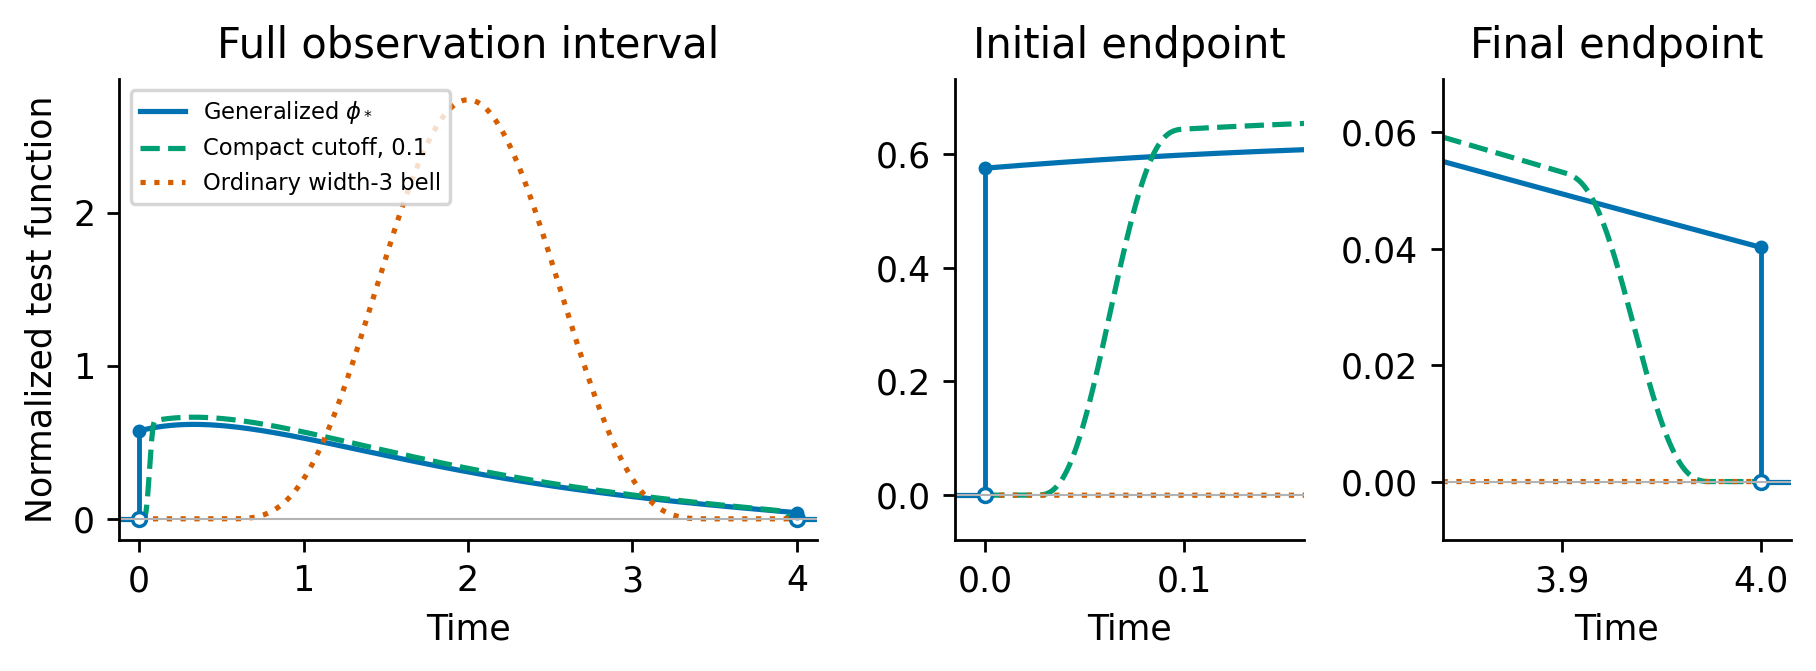
\includegraphics[keepaspectratio,alt={Figure 1. Scalar optimal generalized test for a=-1, x\_0=2, T=4 and \textbackslash tau=0.4, alongside its compact cutoff with width 0.1 and an ordinary width-three bell. All tests use the same clean-moment normalization. Endpoint panels show nonzero one-sided traces and jumps of the zero extension; their adjoint derivatives supply endpoint atoms. The curves describe influences annihilating the initial sensitivity, under the unknown-initial information reference.}]{figures/publication/optimal_test_function.png}}
\caption{Scalar optimal generalized test for \(a=-1\),
\(x_0=2\), \(T=4\) and \(\tau=0.4\), alongside its compact cutoff with
width 0.1 and an ordinary width-three bell. All tests use the same
clean-moment normalization. Endpoint panels show nonzero one-sided
traces and jumps of the zero extension; their adjoint derivatives supply
endpoint atoms. The curves describe influences annihilating the initial
sensitivity, under the unknown-initial information reference.}
\end{figure}

\subsubsection{5.4. Correct-covariance GLS and dense
spans}\label{correct-covariance-gls-and-dense-spans}

For tests \(\phi_k\), put \(\lambda_k=\mathcal D^*\phi_k\),
\(D_{kr}=\langle\lambda_k,S_r\rangle\) and
\(\Sigma_{k\ell}=\langle\lambda_k,C\lambda_\ell\rangle\). Remove exact
linear dependencies. If \(D\) has full column rank, covariance-weighted
weak regression has local influence and covariance

\[
P=(D^T\Sigma^{-1}D)^{-1}D^T\Sigma^{-1},\qquad
V_K=(D^T\Sigma^{-1}D)^{-1}.
\]

WENDy's covariance iteration motivates this construction {[}24{]}, and
physical-OU covariance changes its temporal weights. Under polynomial
features Proposition 4 supplies the complete coupled residual weights.
Its order-one term determines the small-noise efficient influence;
higher orders correct residual uncertainty at finite amplitude without
by themselves removing coefficient-estimator bias.

This is the Godambe-information construction for optimally weighted
estimating equations {[}10{]}: the local information is
\(D^\top\Sigma^{-1}D\). WENDy-MLE has the same leading small-noise map
under regularity and correctly specified covariance; finite-noise
covariance-derivative terms distinguish its objective (S6.3).

\textbf{Proposition 3 (guarded fixed-family weak GLS).} Fix a finite
deterministic boundary-free test family, a correctly specified
polynomial vector field linear in its coefficients, known initial state
and supplied independent-coordinate OU covariance shape. Suppose the
true coefficient is interior to a compact final box; clean and nearby
pilot trajectories exist in a common bounded region; the clean pilot and
final designs have full column rank; and the first-order residual
covariance \(\Sigma_1\) is positive definite. Quadrature weights have
bounded total mass, converge to their integrals, and clean quadrature
and pilot-model numerical defects are \(o(\epsilon)\) with the local
derivative control in (G4) of S7.2.

Use a declared pilot family containing the true vector field and a pilot
box containing its true coefficients. Apply corrected least squares,
clip the pilot, evaluate the full Hermite covariance on its integrated
trajectory, and apply the vanishing-ridge, guarded and box-projected GLS
routine described below. Then its pilot is root-\(\epsilon\) consistent,
its normalized weights converge, and

\[
\epsilon^{-1}(\widehat\theta_{K,\epsilon}-\theta)\Rightarrow N(0,V_K),\qquad
\epsilon^{-2}\operatorname{Cov}(\widehat\theta_{K,\epsilon})\to V_K.
\]

The squared scaled errors are uniformly integrable. These conclusions
are derived from the stated structural and numerical conditions; an
asymptotic expansion, weight consistency and integrability are not
assumed. S7.2 proves the proposition. For nested dense families
satisfying these conditions separately, the subsequent family limit
gives the bound of Theorem 1. Theorem 3 supplies a full-library
smoothed-data construction whose clean ranks follow from a jet condition
instead of being assumed.

The archived solvers in Tables 1--6 use fixed relative ridge and an
unbounded final estimate. Their local matrix geometry and empirical
recovery are separate from the risk guarantee above. For fixed design
\(D\) and residual shape \(\Sigma_1\), their regularized linear map has

\[
W_\rho=[\Sigma_1+\rho\operatorname{tr}(\Sigma_1)I/q]^{-1},\quad
P_\rho=(D^\top W_\rho D)^{-1}D^\top W_\rho,\quad
V_\rho=P_\rho\Sigma_1P_\rho^\top.
\]

Here \(q\) is the number of moments, and \(V_0\) is ideal GLS
covariance. The exact identity

\[
V_\rho-V_0=(P_\rho-P_0)\Sigma_1(P_\rho-P_0)^\top\succeq0
\]

quantifies ridge cost without any estimator-limit assumption. On eight
actual 480-interior-window archived spans and their endpoint/control
extensions, including Lorenz, the largest computed relative RMSE
increment is \(6.7\times10^{-15}\); S7.3 gives the matrices and checks.
Thus the stated ridge has negligible local matrix cost in these
examples. This check cannot establish moments of an unbounded nonlinear
final estimate. Table S8 separates those archived benchmarks, the
constructive estimator and supplied-candidate testing.

\subsubsection{5.5. Extended class and recovery with a known initial
state}\label{extended-class-and-recovery-with-a-known-initial-state}

Throughout this subsection, \(u\) is known exactly, covariance is
supplied and independent of \(\theta\), \(J\) is continuous, and \(S\)
and \(Z\) belong to the OU Cameron--Martin space \(\mathcal H\). Assume
\(\mathcal I_{\theta\theta}\) is positive definite. The coordinate OU
scales and correlation times are positive. Consequently \(\mathcal E\)
is the covariance-dual space of vector-valued \(H^1([0,T])\), with
continuous endpoint evaluation. The initial sensitivity is normalized by
\(Z(0)=I_d\) and the parameter sensitivity satisfies \(S(0)=0\).

For \(\phi\in H^1([0,T];\mathbb R^d)\), use the known-initial residual

\[
m_\phi(\theta)=-\int_0^T[\phi'^TY+\phi^Tf_\theta^H(Y)]dt
+\phi(T)^TY(T)-\phi(0)^Tu.
\]

Its first-order influence is
\(L\phi=(-\phi'-J^T\phi)dt+\phi(T)\delta_T\). The initial boundary term
contains the exact state rather than its noisy observation. This
adaptation of the weak identity is established {[}1{]}. The result below
specifies its covariance-dual geometry and its relation to the
correlated-noise control.

\textbf{Theorem 2 (known-initial extended influence class).} Under these
assumptions,

\[
\overline{L(H^1)}^{\mathcal E}
=\overline{L\{\phi\in H^1:\phi(T)=0\}}^{\mathcal E}
=\mathcal E.
\]

In contrast, allowing only a terminal trace preserves the original
class:

\[
\overline{L\{\phi\in H^1:\phi(0)=0\}}^{\mathcal E}=\mathcal M.
\]

Alternatively, adding the initial noise controls to the closed
boundary-free class gives the exact equality

\[
\mathcal M+\{a\delta_0:a\in\mathbb R^d\}=\mathcal E.
\]

The sharp normalized influence covariance in either full extended
closure is \(\mathcal I_{\theta\theta}^{-1}\), with representative
\(\Lambda_{\mathrm{full}}=C^{-1}S\mathcal I_{\theta\theta}^{-1}\). For
ordinary tests it is an infimum; an exact smooth-test minimum
additionally requires the representative to belong to the specified
range. Explicit initial observation controls can realize the initial
atom.

\emph{Proof.} For \(g\in\mathcal H\), the continuous dual pairing obeys

\[
\langle g,L\phi\rangle
=\int_0^T\phi^T(g'-Jg)dt+\phi(0)^Tg(0).
\]

If this vanishes for all permitted tests, compact interior tests first
imply \(g'=Jg\) in the weak sense. Such solutions are \(g=Zc\). For all
\(H^1\) tests, or for tests with \(\phi(T)=0\), the initial trace is
arbitrary, so \(g(0)=c=0\). Their annihilator is trivial and their
closure is \(\mathcal E\). For tests with \(\phi(0)=0\), every \(Zc\)
annihilates the range and there are no further annihilators. Its closure
is therefore \(\mathcal M\), as characterized in Theorem 1.

For any \(\lambda\in\mathcal E\), define
\(a_j=\langle Z_{\cdot j},\lambda\rangle\). Continuity of this pairing
follows from \(Z\in\mathcal H\). Since \(Z(0)=I_d\),
\(\lambda-a\delta_0\) annihilates every initial-sensitivity column and
belongs to \(\mathcal M\). This proves the exact sum identity. For
covariance optimality, \(\langle\Lambda_{\mathrm{full}},S\rangle=I_p\)
and
\(\operatorname{Cov}(\Lambda_{\mathrm{full}})=\mathcal I_{\theta\theta}^{-1}\).
Any other normalized influence has a covariance-orthogonal remainder,
giving a positive-semidefinite covariance increment. Density, continuous
pairing with \(S\) and normalization by the convergent sensitivity
matrix give attainability as an infimum, by the same approximation
argument as Theorem 1. \(\square\)

Correct-covariance GLS on dense universal extended spans approaches this
bound under the sequential small-noise conditions of Proposition 3, with
the full rather than nuisance-adjusted information. The theorem concerns
the closed local influence class; performance of finite families and
finite-noise covariance pilots requires numerical assessment. In
particular, finite-span gains of different endpoint additions can
overlap.

For compact tests, let \(\Omega\) be the exact Hermite residual
covariance, \(\Sigma_0=\operatorname{diag}(\sigma_j^2)\) and
\(B=\operatorname{Cov}(m_\phi,Y(0)-u)\). The optimal linear control
replaces the residual covariance by

\[
\Omega-B\Sigma_0^{-1}B^T.
\]

Only the first Hermite order contributes to \(B\). In coordinate \(j\),
its cross-covariance is the integral of the linear residual weight
against \(\sigma_j^2e^{-t/\tau_j}\). In a sampled iid model the
compact-test weights and derivatives vanish at the initial node; hence
this cross-covariance is exactly zero. This distinction explains the
correlated-noise control mechanism. It does not establish an additional
finite-family gain when initial-trace tests already approximate the full
efficient directions.

\subsubsection{5.6. Constructive full-library
attainability}\label{constructive-full-library-attainability}

This is a constructive attainability result: the algorithm witnesses the
sharp small-noise bound. Its moderate-noise precision is assessed
separately in Section 7.6. The following procedure estimates every
supplied library coefficient. Let \(B\) be the compact coefficient box
and use uniform grids with an even number of intervals. Smooth the
linear interpolant of \(Y\) with

\[
\begin{aligned}
K_b(t)&=b^{-1}(315/256)[1-(t/b)^2]_+^4,\quad b=\epsilon^{1/10}/4,\\
w(t)&=[1-((t-T/2)/(T/2-1/2))^2]_+^4.
\end{aligned}
\]

Reflect the interpolant at the endpoints. The proxy \(z\) supplies the
\(m\) feature tests \(w g_j(z)\) and their analytic derivatives. Their
Hermite-corrected weak equations give a full-library least-squares
pilot, clipped to \(B\). A fixed deterministic-window pilot on a
declared correct structural family gives the alternative construction in
Proposition 3.

Append the cubic splines \(B_3(t/a-j)\), \(a=T/2^k\),
\(j=2,\ldots,2^k-2\), where \(B_3\) is the normalized cardinal cubic
spline supported on \([-2,2]\). Whiten the combined \(H^1\) Gram matrix,
retaining eigenvalues above \(10^{-10}\epsilon^{1/10}\) times its
largest eigenvalue. The exact Hermite covariance (Proposition 4),
evaluated at the proxy and pilot, gives
\(\widehat\Sigma_1=\widehat\Omega/\epsilon^2\). Add ridge
\(\epsilon^2\operatorname{tr}(\widehat\Sigma_1)I/q\), then solve
corrected GLS and project the result to \(B\). Relative
minimum-eigenvalue guards use \(10^{-8}\epsilon^2\); singular, nonfinite
or failed calculations return the box midpoint. S8 specifies the column
scaling and covariance guard. No generating support or pilot ODE
solution is supplied to this full-library procedure.

The technical restriction \(T>1\) makes the fixed half-unit interior
margins of \(w\) nonempty. Proportional margins and a rescaled kernel
give an equivalent construction on any positive horizon. Write
\(\mathcal I_{e,C}\) for the initial-state-adjusted information of
Theorem 1 computed with the unit-amplitude covariance \(C\) of \(\eta\).

\textbf{Theorem 3 (constructive attainability under a jet condition).}
Consider an analytic trajectory \(x_0\) of a polynomial ODE on
\([0,T]\), \(T>1\), with vector field linear in a polynomial library
\(g_1,\ldots,g_m\) in each of \(d\) equations. Let the \(dm\) true
coefficients lie strictly inside a supplied compact box. Observe
\(Y=x_0+\epsilon\eta\) with known positive independent-coordinate
stationary OU covariance. Assume that, at some \(t_*\) in the
observation interval,

\[
\det[\partial_t^r g_j(x_0(t_*))]_{r=0,\ldots,m-1;\ j=1,\ldots,m}\ne0.
\]

For the full-library procedure just defined, let \(h^2=o(\epsilon)\).
For each fixed spline level \(k\), the pilot is root-\(\epsilon\)
consistent, the normalized covariance weights are consistent, and

\[
\epsilon^{-1}(\widehat\theta_{k,\epsilon}-\theta_0)\Rightarrow N(0,V_k),\qquad
\epsilon^{-2}E[(\widehat\theta_{k,\epsilon}-\theta_0)(\widehat\theta_{k,\epsilon}-\theta_0)^\top]\to V_k.
\]

The squared scaled errors are uniformly integrable, and
\(V_k\to\mathcal I_{e,C}^{-1}\) as \(k\to\infty\) after the fixed-level
small-noise limit. The coefficient pilot uses all library terms; no
generating support is supplied. S8.1 proves the general result,
including rank, weight consistency and moment control; S8.2 verifies it
for Van der Pol with the full 18-coefficient cubic library and
\(u=(2,0)\), where the jet determinant is \(-65265167726360395776\).
This theorem concerns the specified guarded estimator and sequential
limits, not finite-noise Wald calibration or the archived fixed-ridge
fits.

\subsection{6. Exact polynomial weak-residual
covariance}\label{exact-polynomial-weak-residual-covariance}

\subsubsection{6.1. Finite Hermite
expansion}\label{finite-hermite-expansion}

Assume a common \(\tau\) for independent coordinates, and set
\(v_j=\sigma_j^2\). Define \(H_0(z;v)=1\), \(H_1(z;v)=z\),
\(H_{q+1}(z;v)=zH_q(z;v)-qvH_{q-1}(z;v)\) and corrected monomials
\(\widetilde\vartheta_\beta(y)=\prod_jH_{\beta_j}(y_j;v_j)\). Their
expectation given \(x\) is \(x^\beta\). This Gaussian debiasing
construction {[}27{]} centers the polynomial residual at the true
coefficients.

For continuum residual \(r_{ki}=b_{ki}-(G\xi^*)_{ki}\), polynomial
expansion gives

\[
r_{ki}=\sum_{1\leq|\alpha|\leq p_*}\int_0^Tc_{ki,\alpha}(t)H_\alpha(\eta_C(t);v)dt,
\]

where \(p_*\geq1\) is the relevant maximum degree,
\(H_\alpha=\prod_jH_{\alpha_j}\) and

\[
c_{ki,\alpha}=-\mathbf1_{\{\alpha=e_i\}}\phi'_k
-\phi_k\frac{\partial^\alpha f_i(x)}{\alpha!}.
\]

The response and feature perturbations share this coefficient and retain
their cross-covariance.

\textbf{Proposition 4 (exact covariance).} Under these assumptions,

\[
\operatorname{Cov}(r_{ki},r_{\ell m})=
\sum_{1\leq|\alpha|\leq p_*}\alpha!\prod_jv_j^{\alpha_j}
\int_0^T\int_0^Tc_{ki,\alpha}(s)c_{\ell m,\alpha}(t)
e^{-|\alpha||s-t|/\tau}\,ds\,dt.
\]

\textbf{Proof.} The generating function \(\exp(az-va^2/2)\) yields
\(E[H_q(U;v)H_r(V;v)]=\mathbf1_{q=r}q!v^q\rho^q\) for jointly Gaussian
variables of variance \(v\) and correlation \(\rho\). This is the
Hermite form of classical Gaussian moment identities {[}36{]}.
Coordinate independence gives orthogonality between different
multi-indices and factor \(\alpha!\prod_jv_j^{\alpha_j}\). Substitute
\(\rho=e^{-|s-t|/\tau}\) and integrate the finite expansion. \(\square\)

The order-one covariance supplies the GLS weights required by
Proposition 3. Higher orders refine residual weights at finite
amplitude; coefficient bias also depends on random-design terms. Order
\(q\) has correlation time \(\tau/q\). Higher orders need not be
negligible at moderate amplitude. Different windows and equations remain
correlated despite independent sensor coordinates. The covariance is
exact for a supplied clean trajectory and true polynomial; plugging in
estimates introduces another approximation.

\subsubsection{6.2. Implementation and covariance
misspecification}\label{implementation-and-covariance-misspecification}

The finite Hermite sum can be evaluated on a grid without storing a
dense temporal matrix. S6.4 gives the recursion and the extension to
incorrectly corrected raw features. Under temporal weights \(W\),
leading covariance is \(P_W\Sigma_{\mathrm{true},1}P_W^\top\); changing
correction variances can also change the moment mean. The present
comparisons supply the sensor covariance. Sensitivity to supplied and
fitted correlation times is reported in S5.4.

\subsection{7. Numerical benchmarks: cost, recovery and
attainability}\label{numerical-benchmarks-cost-recovery-and-attainability}

The benchmarks use fully observed polynomial systems, supplied structure
and sensor covariance, and archived paired observations. Feasible
covariance pilots receive no generating coefficients. S2--S5 preserve
protocols, seed ranges, fingerprints and additional checks. Local
references and finite-noise performance are reported separately.

\subsubsection{7.1. Information cost and finite-span
efficiency}\label{information-cost-and-finite-span-efficiency}

For Van der Pol, we fit four independent coefficients in \(x'=av\),
\(v'=bx+cv+dx^2v\), with truth \((1,-1,1,-1)\), initial state \((2,0)\),
\(T=20\), \(h=0.005\) and OU range 0.3. Relative errors are divided by
the true coefficient norm, two. The known-initial local RMSE reference
at 5\% noise is 0.013093, versus the boundary-free reference 0.016904: a
29\% cost. Both scale linearly with noise amplitude.

\begin{center}
\begin{minipage}{\linewidth}
Table 1. Oracle Gaussian influence RMSE under actual OU noise at 5\%.
Both methods use the same test span and clean design; they differ only
in the covariance used for GLS weights. Actual variance uses the OU
covariance for both.

\small\setlength{\tabcolsep}{3pt}
\begin{tabular}{@{}
  >{\raggedleft\arraybackslash}p{(\linewidth - 8\tabcolsep) * \real{0.2000}}
  >{\raggedleft\arraybackslash}p{(\linewidth - 8\tabcolsep) * \real{0.2000}}
  >{\raggedleft\arraybackslash}p{(\linewidth - 8\tabcolsep) * \real{0.2000}}
  >{\raggedleft\arraybackslash}p{(\linewidth - 8\tabcolsep) * \real{0.2000}}
  >{\raggedleft\arraybackslash}p{(\linewidth - 8\tabcolsep) * \real{0.2000}}@{}}
\toprule\noalign{}
\begin{minipage}[b]{\linewidth}\raggedleft
Prescribed windows
\end{minipage} & \begin{minipage}[b]{\linewidth}\raggedleft
Retained tests
\end{minipage} & \begin{minipage}[b]{\linewidth}\raggedleft
OU-weight RMSE
\end{minipage} & \begin{minipage}[b]{\linewidth}\raggedleft
iid-weight RMSE
\end{minipage} & \begin{minipage}[b]{\linewidth}\raggedleft
OU RMSE / class reference
\end{minipage} \\
\midrule\noalign{}
30 & 30 & 0.019605 & 0.020296 & 1.1597 \\
120 & 120 & 0.017043 & 0.017839 & 1.0082 \\
480 & 479 & 0.016938 & 0.017734 & 1.0020 \\
\bottomrule
\end{tabular}
\end{minipage}
\end{center}

Rich spans produce most of the improvement: 480-window OU GLS is within
0.2\% of the boundary-free local reference, while iid weights retain a
roughly 5\% gap. Exact residual-covariance calculations verify the
stated local geometry. The original 128-path finite-span check is in
S5.2; the larger paired comparison follows.

\begin{center}
\begin{minipage}{\linewidth}
Table 2. Van der Pol on the same 2000 paths at 0.5\% noise. Error norms
are divided by the true four-coefficient norm, two. The reference
concerns the leading local Gaussian influence. All paths are retained.

\small\setlength{\tabcolsep}{3pt}
\begin{tabular}{@{}
  >{\raggedright\arraybackslash}p{(\linewidth - 8\tabcolsep) * \real{0.1579}}
  >{\raggedleft\arraybackslash}p{(\linewidth - 8\tabcolsep) * \real{0.2105}}
  >{\raggedleft\arraybackslash}p{(\linewidth - 8\tabcolsep) * \real{0.2105}}
  >{\raggedleft\arraybackslash}p{(\linewidth - 8\tabcolsep) * \real{0.2105}}
  >{\raggedleft\arraybackslash}p{(\linewidth - 8\tabcolsep) * \real{0.2105}}@{}}
\toprule\noalign{}
\begin{minipage}[b]{\linewidth}\raggedright
Estimator
\end{minipage} & \begin{minipage}[b]{\linewidth}\raggedleft
RMSE (95\% interval)
\end{minipage} & \begin{minipage}[b]{\linewidth}\raggedleft
Bias
\end{minipage} & \begin{minipage}[b]{\linewidth}\raggedleft
Dispersion
\end{minipage} & \begin{minipage}[b]{\linewidth}\raggedleft
Local reference
\end{minipage} \\
\midrule\noalign{}
One step, known initial & 0.001301 {[}0.001269, 0.001332{]} & 0.000085 &
0.001298 & 0.001309 \\
One step, unknown initial & 0.001838 {[}0.001790, 0.001887{]} & 0.000469
& 0.001777 & 0.001690 \\
Three steps, unknown initial & 0.001669 {[}0.001630, 0.001708{]} &
0.000068 & 0.001668 & 0.001690 \\
Weak GLS, OU & 0.001685 {[}0.001645, 0.001723{]} & 0.000083 & 0.001683 &
0.001690 \\
Weak GLS, iid & 0.001759 {[}0.001718, 0.001801{]} & 0.000103 & 0.001756
& 0.001690 \\
\bottomrule
\end{tabular}
\end{minipage}
\end{center}

All 2000 prespecified paths at 0.5\% noise are retained, including the
original 128-path prefix once. Feasible weak GLS uses a bounded
30-window covariance pilot and 480 prescribed windows. Likelihood
refinements use exact OU innovations and analytical ODE sensitivities.
Paired iid-minus-OU RMSE is 0.00007426, with bootstrap interval
{[}0.00005576, 0.00009327{]}, a 4.22\% benefit from temporal weighting.
The initial unknown-state scoring step has an appreciable nonlinear
initialization bias; three steps approach the nuisance-adjusted
reference. The known-initial estimate has lower error because it
observes the information discarded by compact tests.

\begin{figure}[p]
\centering
\pandocbounded{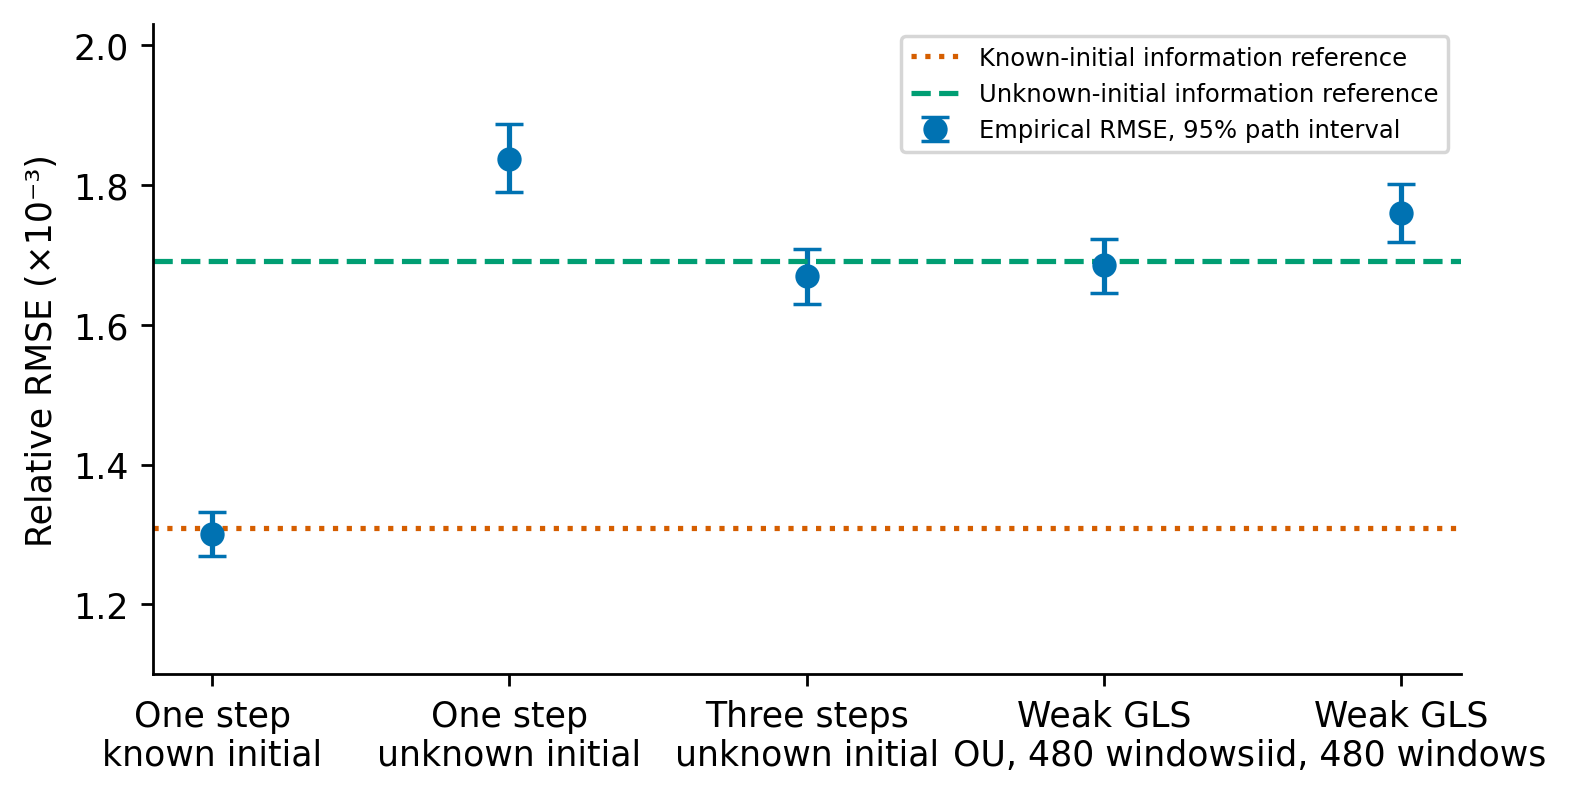
\includegraphics[keepaspectratio,alt={Figure 2. Van der Pol on 2000 shared paths at 0.5\% noise: one scoring step with known initial state, one or three joint steps with unknown initial state, and weak GLS with OU or iid weights. Whiskers give 95\% bootstrap intervals for RMSE over independent paths, not parameter confidence intervals or error standard deviations. The known-initial information reference is lower than the unknown-initial reference. The finite-step unknown-initial estimates are identified separately; reference agreement concerns local small-noise behavior.}]{figures/publication/likelihood_comparison.png}}
\caption{Van der Pol on 2000 shared paths at 0.5\% noise: one
scoring step with known initial state, one or three joint steps with
unknown initial state, and weak GLS with OU or iid weights. Whiskers
give 95\% bootstrap intervals for RMSE over independent paths, not
parameter confidence intervals or error standard deviations. The
known-initial information reference is lower than the unknown-initial
reference. The finite-step unknown-initial estimates are identified
separately; reference agreement concerns local small-noise behavior.}
\end{figure}

\subsubsection{7.2. Recovery with universal endpoint
tests}\label{recovery-with-universal-endpoint-tests}

For known \(u\), allow nonzero test traces and use the corrected
residual

\[
m_\phi(\theta)=-\int_0^T[\phi'(t)^TY(t)+\phi(t)^Tf_\theta^H(Y(t))]dt
+\phi(T)^TY(T)-\phi(0)^Tu.
\]

The universal family adds twelve time-only endpoint half-windows and
\(Y(0)-u\) controls to 480 interior windows. Covariance weights still
require an integrated 30-window pilot. Theorem 2 identifies the full
local influence class; the known-initial trace adaptation itself is
established by Brunel et al. {[}1{]}.

\begin{center}
\begin{minipage}{\linewidth}
Table 3. Known-initial endpoint confirmation on 1968 paired Van der Pol
paths at 0.5\% noise. The likelihood reference is one Fisher-scoring
step. All errors use the four-coefficient norm, two.

\small\setlength{\tabcolsep}{3pt}
\begin{tabular}{@{}lrrr@{}}
\toprule\noalign{}
Method & RMSE & Bias norm & Dispersion \\
\midrule\noalign{}
Boundary-free, 480 & 0.00168754 & 0.00008679 & 0.00168531 \\
Universal endpoints & 0.00130936 & 0.00007049 & 0.00130746 \\
Model-adjoint endpoints & 0.00129741 & 0.00006771 & 0.00129564 \\
Known-initial scoring & 0.00129800 & 0.00008753 & 0.00129505 \\
\bottomrule
\end{tabular}
\end{minipage}
\end{center}

These 1968 records were unused for endpoint fitting, while their compact
and scoring references were archived. After inspecting the 32-path
pilot, we replaced the absolute RMSE gate of 0.00140 with paired
relative criteria because known-initial likelihood itself failed that
gate; the amendment was frozen before any new endpoint outcomes on the
1968 confirmation records were inspected. The frozen confirmation
criterion requires at least 50\% gap recovery. Universal endpoints
recover 97.1\%, with paired interval 95.5--98.6\%, and lie 0.88\% above
scoring. Model-adjoint tests realize score directions and provide an
implementation check. S2 and S5.5 record the criterion amendment and
quadrature checks.

\begin{figure}[p]
\centering
\pandocbounded{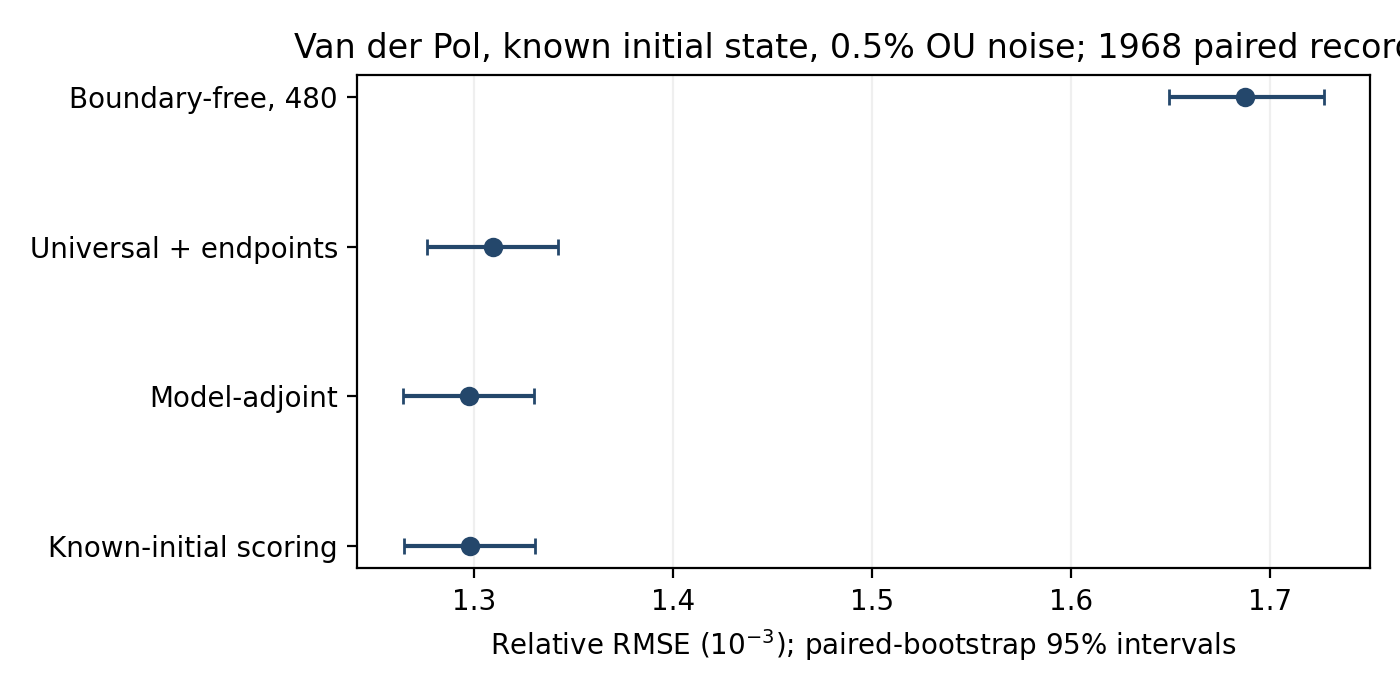
\includegraphics[keepaspectratio,alt={Figure 3. Known-initial information recovery on 1968 paired Van der Pol records at 0.5\% OU noise. Whiskers are Monte Carlo 95\% RMSE intervals from shared record bootstrap resamples. Universal time-only endpoint windows recover 97.1\% of the original weak-to-scoring gap; model-adjoint tests serve as a score-realization check. The reference is a single known-initial Fisher-scoring step.}]{figures/publication/endpoint_confirmation.png}}
\caption{Known-initial information recovery on 1968 paired Van
der Pol records at 0.5\% OU noise. Whiskers are Monte Carlo 95\% RMSE
intervals from shared record bootstrap resamples. Universal time-only
endpoint windows recover 97.1\% of the original weak-to-scoring gap;
model-adjoint tests serve as a score-realization check. The reference is
a single known-initial Fisher-scoring step.}
\end{figure}

\subsubsection{7.3. Attribution to initial
traces}\label{attribution-to-initial-traces}

The 500-path ablation holds Simpson quadrature and the covariance pilot
fixed. Component gains are measured against the matched compact branch
and known-initial scoring.

\begin{center}
\begin{minipage}{\linewidth}
Table 4. Endpoint-component ablation on 500 paired paths at 0.5\% noise.
Recovery is measured against the matched Simpson boundary-free branch
and known-initial scoring. Intervals resample common record indices.

\small\setlength{\tabcolsep}{3pt}
\begin{tabular}{@{}lrrr@{}}
\toprule\noalign{}
Added component & RMSE & Gap closed & Paired 95\% interval \\
\midrule\noalign{}
Initial half-windows & 0.00132445 & 98.9\% & {[}95.1\%; 102.7\%{]} \\
Terminal half-windows & 0.00164493 & -0.3\% & {[}-1.8\%; 1.2\%{]} \\
Initial controls only & 0.00159795 & 14.3\% & {[}7.0\%; 21.4\%{]} \\
All components & 0.00132453 & 98.9\% & {[}95.1\%; 102.6\%{]} \\
Matched boundary-free & 0.00164395 & 0\% & --- \\
Known-initial scoring & 0.00132100 & 100\% & --- \\
\bottomrule
\end{tabular}
\end{minipage}
\end{center}

Initial traces alone recover essentially the entire gap, quantifying the
Brunel mechanism under OU noise. Initial controls give a smaller
standalone gain and terminal traces give none resolved. Combining all
components changes RMSE relative to initial traces by
\(7.46\times10^{-8}\), with paired interval
\([-7.18\times10^{-7},8.55\times10^{-7}]\). Their contributions overlap
and cannot be added. The control's standalone improvement is specific to
correlation between initial and interior error, rather than evidence for
an additional gain after trace adaptation.

\begin{figure}[p]
\centering
\pandocbounded{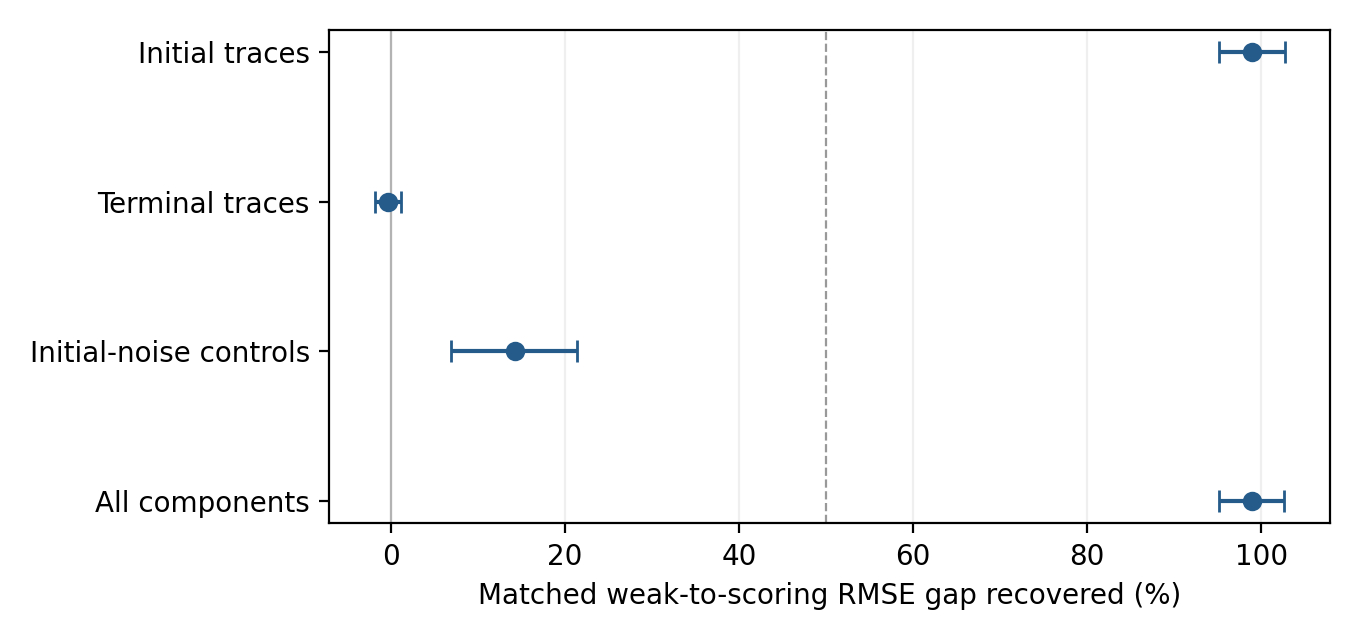
\includegraphics[keepaspectratio,alt={Figure 4. Paired endpoint-component attribution on 500 Van der Pol records. Whiskers show 95\% bootstrap intervals for the fraction of the matched weak-to-scoring RMSE gap recovered. The dashed line marks the prespecified 50\% material-contribution rule. Initial traces recover the gap; initial-noise controls give a smaller standalone gain, and terminal traces give no resolved improvement. Contributions overlap.}]{figures/publication/endpoint_ablation.png}}
\caption{Paired endpoint-component attribution on 500 Van der
Pol records. Whiskers show 95\% bootstrap intervals for the fraction of
the matched weak-to-scoring RMSE gap recovered. The dashed line marks
the prespecified 50\% material-contribution rule. Initial traces recover
the gap; initial-noise controls give a smaller standalone gain, and
terminal traces give no resolved improvement. Contributions overlap.}
\end{figure}

\subsubsection{7.4. Moderate-noise limits and Lorenz
confirmation}\label{moderate-noise-limits-and-lorenz-confirmation}

The 5\% Van der Pol check reuses all 128 matched observations, with
known initial state and the same feasible pilot. The likelihood
reference optimizes exact OU innovations.

\begin{center}
\begin{minipage}{\linewidth}
Table 5. Moderate-noise endpoint confirmation on 128 paired Van der Pol
paths at 5\%. The known-initial reference uses full nonlinear likelihood
fitting.

\small\setlength{\tabcolsep}{3pt}
\begin{tabular}{@{}lrrr@{}}
\toprule\noalign{}
Method & RMSE & Bias norm & Dispersion \\
\midrule\noalign{}
Matched boundary-free & 0.0255965 & 0.0081646 & 0.0242594 \\
Universal endpoints & 0.0218790 & 0.0056954 & 0.0211247 \\
Known-initial MLE & 0.0142088 & 0.0007255 & 0.0141902 \\
Unknown-initial MLE & 0.0171952 & 0.0006504 & 0.0171829 \\
\bottomrule
\end{tabular}
\end{minipage}
\end{center}

Universal endpoints recover 32.6\% of the gap (18.3--45.8\%), failing
the frozen 50\% criterion. Clean-design first-order and full-Hermite
references are 0.013094 and 0.013636, below empirical dispersion
0.021125. Restored local geometry therefore leaves finite-noise design,
pilot and fitting effects. The matched author-WENDy comparison is in
S5.3.

For Lorenz, we fit \((s,r,b)=(10,28,8/3)\) in its supplied physical
structure, with \(u=(1,1,1)\), \(T=4\), \(h=0.001\), OU range 0.1 and
0.5\% coordinate noise. The unknown-initial local relative RMSE
reference is 0.000411, versus 0.000209 when the initial state is known:
almost a factor two.

\begin{center}
\begin{minipage}{\linewidth}
Table 6. Lorenz endpoint confirmation on 256 paired paths. Errors are
relative to the norm of \((10,28,8/3)\). The common horizon is four and
the sampling interval is 0.001.

\small\setlength{\tabcolsep}{3pt}
\begin{tabular}{@{}lrrr@{}}
\toprule\noalign{}
Method & RMSE & Bias norm & Dispersion \\
\midrule\noalign{}
Matched boundary-free & 0.00040994 & 0.00002170 & 0.00040936 \\
Universal endpoints & 0.00021686 & 0.00002153 & 0.00021579 \\
Known-initial MLE & 0.00020784 & 0.00002355 & 0.00020650 \\
\bottomrule
\end{tabular}
\end{minipage}
\end{center}

All 256 paths and all converged fits are retained. Universal endpoint
windows recover 95.5\% of the compact-to-likelihood gap (92.8--98.0\%),
passing the same 50\% rule. The full-Hermite clean-design reference is
0.00020926, close to the observed endpoint dispersion. These two
supplied structures support small-noise recovery; moderate-noise
universality remains unestablished.

\subsubsection{7.5. Direction-specific information
cost}\label{direction-specific-information-cost}

For the prespecified negative cubic perturbation \(\delta x^3\) in the
second Van der Pol equation, profiling all seventeen other library
coefficients gives local full-information and boundary-free two-point
reference magnitudes 0.01928 and 0.01941 at 0.5\% noise. The
initial-state information cost for this direction is only 0.68\%,
despite its larger aggregate coefficient-estimation cost.
Supplied-candidate Wald testing and library-wide sparse selection have
different inputs and targets; their detailed comparison and calibration
studies are supplementary (S3, S4 and S9).

\subsubsection{7.6. Matching the constructive estimator to its
finite-span
reference}\label{matching-the-constructive-estimator-to-its-finite-span-reference}

The full-library estimator of Theorem 3 uses nine smoothed-data feature
instruments and 125 time-only cubic splines. The deterministic limiting
covariance for this 134-test span has
\(\sqrt{\operatorname{tr}V_k}=9.8144\). The calculation retains all rows
and uses neither ridge nor rank truncation. Refining the finest grid
from \(h=0.00015625\) to \(0.000078125\) changes this reference by
\(4.7\times10^{-8}\) relatively. It concerns all eighteen coefficients,
unlike the earlier supplied four-coefficient Van der Pol benchmarks.

\begin{center}
\begin{minipage}{\linewidth}
Table 7. Constructive full-library estimator on 100 independent paths at
each amplitude. Intervals resample archived coefficient errors 10,000
times and are pointwise; no new observations are generated for this
comparison.

\small\setlength{\tabcolsep}{3pt}
\begin{tabular}{@{}
  >{\raggedleft\arraybackslash}p{(\linewidth - 6\tabcolsep) * \real{0.2500}}
  >{\raggedleft\arraybackslash}p{(\linewidth - 6\tabcolsep) * \real{0.2500}}
  >{\raggedleft\arraybackslash}p{(\linewidth - 6\tabcolsep) * \real{0.2500}}
  >{\raggedleft\arraybackslash}p{(\linewidth - 6\tabcolsep) * \real{0.2500}}@{}}
\toprule\noalign{}
\begin{minipage}[b]{\linewidth}\raggedleft
Noise
\end{minipage} & \begin{minipage}[b]{\linewidth}\raggedleft
RMSE/\(\epsilon\)
\end{minipage} & \begin{minipage}[b]{\linewidth}\raggedleft
RMSE/\((\epsilon\sqrt{\operatorname{tr}V_k})\)
\end{minipage} & \begin{minipage}[b]{\linewidth}\raggedleft
95\% interval for ratio
\end{minipage} \\
\midrule\noalign{}
5\% & 11.6265 & 1.1846 & 1.1140--1.2563 \\
0.5\% & 10.3505 & 1.0546 & 0.9883--1.1202 \\
0.1\% & 9.9850 & 1.0174 & 0.9452--1.0885 \\
0.05\% & 9.5899 & 0.9771 & 0.8994--1.0528 \\
0.01\% & 9.3516 & 0.9528 & 0.8891--1.0147 \\
\bottomrule
\end{tabular}
\end{minipage}
\end{center}

All four lower-noise ratio intervals include one; the 5\% interval lies
above it. There are no guard fallbacks or final clipping on these 500
paths. The reference uses the full limiting span of 134 tests. At the
four larger amplitudes every fit retains 134 tests; at 0.01\% noise, 65
fits retain 133 and 35 retain 132. Finite-amplitude cutoff and
adaptive-instrument effects therefore remain, and the ratios establish
compatibility with the limiting reference rather than numerical proof of
its attainment. At 5\% noise the total eighteen-coefficient RMSE is
0.5813, or root-mean-square coordinate error 0.1370. At this amplitude
the coordinate error limits practical precision: Theorem 3 establishes
attainability in the small-noise limit, and this construction is an
asymptotic benchmark rather than a recommended moderate-noise fitting
method. Each level has only 100 paths; the intervals leave the apparent
lower-noise trend unresolved. Supplement S9.2 records matrix checks and
covariance diagnostics; Table S8 distinguishes the estimators.

\subsection{8. Discussion and
limitations}\label{discussion-and-limitations}

Boundary-free equations retain exactly the local information available
when the initial state is a nuisance parameter. Their restriction has a
quantified cost when the state is known: 29\% in the Van der Pol
aggregate RMSE reference and almost a factor two for Lorenz. Rich spans
and correct temporal weights approximate the sharp class reference.
Theorem 2 supplies the complementary full-information class for
known-initial boundary adaptations. The exact adjoint-range equalities,
rather than classical projection formulas or the Brunel remedy, are the
theoretical contribution.

The recovery experiment and ablation distinguish class theory from
method novelty. Universal endpoint windows recover 97.1\% of the
weak-to-scoring gap on 1968 Van der Pol records and 95.5\% of the
weak-to-likelihood gap on 256 Lorenz records. On the 500-record Van der
Pol ablation, initial traces alone explain essentially all that gain,
reproducing the established Brunel adaptation. The correlated-noise
initial control is useful separately, recovering 14.3\% of the gap, but
contributes no resolved improvement after initial traces. Thus the
remedy is an established boundary mechanism with a quantitative OU
benchmark. At 5\% Van der Pol noise only 32.6\% of the likelihood gap is
recovered. Covariance weights still require an integrated pilot model;
computational superiority has not been demonstrated.

Information loss is direction specific: initial-state projection raises
the local cubic-candidate detection reference by only 0.68\%, compared
with the larger aggregate coefficient-estimation cost. The supplementary
testing study distinguishes prespecified candidates from unrestricted
structure discovery. The main empirical attainability check instead
matches the full-library estimator to its own finite-span covariance,
with uncertainty reported for the limited 100-path samples. At moderate
noise this large library remains imprecise, and the local theorem does
not establish finite-noise inferential calibration.

The scope is fully observed deterministic polynomial ODEs with known
positive sensor covariance. Small-noise influence efficiency,
finite-noise feasible accuracy and support selection are separate
claims. Exact residual covariance does not by itself give exact
finite-noise estimator variance when weights and designs depend on the
record. On the matched moderate-noise benchmark, likelihood is more
accurate than the original boundary-free weak estimator.
Independent-record GMM, fission and cross-fitting are preserved in the
separate research archive and lie outside the main claims. Joint
span/noise rates, unknown-covariance calibration with heterogeneous
states, partial observation and process noise require further analysis.

\subsection{Data availability}\label{data-availability}

The preceding benchmark is publicly archived in the
\href{https://github.com/malyshevdanil/wsindy-information-limits/tree/v1.2.0}{reproducibility
repository, version v1.2.0} and its
\href{https://doi.org/10.5281/zenodo.23313935}{Zenodo snapshot}. The
present endpoint, selection and SE-calibration follow-ups are preserved
separately in the accompanying reproducibility bundle; the v1.2.0 DOI
identifies the preceding version. Configurations, seed ranges, source
fingerprints, coefficient estimates, covariance summaries and SHA256
manifests permit exact input reconstruction and paired audit. Full
synthetic time series are regenerated from the frozen seed protocol.
Pinned download specifications retrieve original author sources. No
external experimental dataset is used. A public versioned identifier for
the current bundle must be added before submission.

\subsection*{References}\label{references}
\addcontentsline{toc}{subsection}{References}

\protect\phantomsection\label{refs}
\begin{CSLReferences}{0}{0}
\bibitem[\citeproctext]{ref-brunel2014}
\CSLLeftMargin{{[}1{]} }%
\CSLRightInline{{Brunel NJ-B, Clairon Q, d'Alche-Buc F}. Parametric
estimation of ordinary differential equations with orthogonality
conditions. \emph{Journal of the American Statistical Association} 109
(2014) 173--185. \url{https://doi.org/10.1080/01621459.2013.841583}.}

\bibitem[\citeproctext]{ref-heitzman2026}
\CSLLeftMargin{{[}2{]} }%
\CSLRightInline{Heitzman-Breen N, Dukic V, Bortz DM. A practical
identifiability criterion leveraging weak-form parameter estimation.
\emph{Bulletin of Mathematical Biology} 88 (2026) 70.
\url{https://doi.org/10.1007/s11538-026-01639-x}.}

\bibitem[\citeproctext]{ref-brunton2016}
\CSLLeftMargin{{[}3{]} }%
\CSLRightInline{Brunton SL, Proctor JL, Kutz JN. Discovering governing
equations from data by sparse identification of nonlinear dynamical
systems. \emph{Proceedings of the National Academy of Sciences} 113
(2016) 3932--3937. \url{https://doi.org/10.1073/pnas.1517384113}.}

\bibitem[\citeproctext]{ref-schaeffer2017}
\CSLLeftMargin{{[}4{]} }%
\CSLRightInline{Schaeffer H, McCalla SG. Sparse model selection via
integral terms. \emph{Physical Review E} 96 (2017) 023302.
\url{https://doi.org/10.1103/PhysRevE.96.023302}.}

\bibitem[\citeproctext]{ref-messenger2021}
\CSLLeftMargin{{[}5{]} }%
\CSLRightInline{Messenger DA, Bortz DM. Weak {SINDy}: Galerkin-based
data-driven model selection. \emph{Multiscale Modeling and Simulation}
19 (2021) 1474--1497. \url{https://doi.org/10.1137/20M1343166}.}

\bibitem[\citeproctext]{ref-reinbold2020}
\CSLLeftMargin{{[}6{]} }%
\CSLRightInline{Reinbold PAK, Gurevich DR, Grigoriev RO. Using noisy or
incomplete data to discover models of spatiotemporal dynamics.
\emph{Physical Review E} 101 (2020) 010203.
\url{https://doi.org/10.1103/PhysRevE.101.010203}.}

\bibitem[\citeproctext]{ref-stein1999}
\CSLLeftMargin{{[}7{]} }%
\CSLRightInline{Stein ML. Interpolation of spatial data: Some theory for
kriging. Springer (1999)
\url{https://doi.org/10.1007/978-1-4612-1494-6}.}

\bibitem[\citeproctext]{ref-ying1991}
\CSLLeftMargin{{[}8{]} }%
\CSLRightInline{Ying Z. Asymptotic properties of a maximum likelihood
estimator with data from a gaussian process. \emph{Journal of
Multivariate Analysis} 36 (1991) 280--296.
\url{https://doi.org/10.1016/0047-259X(91)90062-7}.}

\bibitem[\citeproctext]{ref-zhang2004}
\CSLLeftMargin{{[}9{]} }%
\CSLRightInline{Zhang H. Inconsistent estimation and asymptotically
equal interpolations in model-based geostatistics. \emph{Journal of the
American Statistical Association} 99 (2004) 250--261.
\url{https://doi.org/10.1198/016214504000000241}.}

\bibitem[\citeproctext]{ref-godambe1960}
\CSLLeftMargin{{[}10{]} }%
\CSLRightInline{Godambe VP. An optimum property of regular maximum
likelihood estimation. \emph{The Annals of Mathematical Statistics} 31
(1960) 1208--1211. \url{https://doi.org/10.1214/aoms/1177705693}.}

\bibitem[\citeproctext]{ref-bickel1993}
\CSLLeftMargin{{[}11{]} }%
\CSLRightInline{Bickel PJ, Klaassen CAJ, Ritov Y, Wellner JA.
\href{https://faculty.washington.edu/jonw/RESEARCH/BOOKS/book3.html}{Efficient
and adaptive estimation for semiparametric models}. Johns Hopkins
University Press (1993).}

\bibitem[\citeproctext]{ref-vandervaart1998}
\CSLLeftMargin{{[}12{]} }%
\CSLRightInline{{van der Vaart AW}. Asymptotic statistics. Cambridge
University Press (1998) \url{https://doi.org/10.1017/CBO9780511802256}.}

\bibitem[\citeproctext]{ref-dette2016}
\CSLLeftMargin{{[}13{]} }%
\CSLRightInline{Dette H, Pepelyshev A, Zhigljavsky A. Optimal designs in
regression with correlated errors. \emph{The Annals of Statistics} 44
(2016) 113--152. \url{https://doi.org/10.1214/15-AOS1361}.}

\bibitem[\citeproctext]{ref-dette2017}
\CSLLeftMargin{{[}14{]} }%
\CSLRightInline{Dette H, Konstantinou M, Zhigljavsky A. A new approach
to optimal designs for correlated observations. \emph{The Annals of
Statistics} 45 (2017) 1579--1608.
\url{https://doi.org/10.1214/16-AOS1500}.}

\bibitem[\citeproctext]{ref-messenger2025}
\CSLLeftMargin{{[}15{]} }%
\CSLRightInline{Messenger DA, Bortz DM. Asymptotic consistency of the
{WSINDy} algorithm in the limit of continuum data. \emph{IMA Journal of
Numerical Analysis} 45 (2025) 3264--3312.
\url{https://doi.org/10.1093/imanum/drae086}.}

\bibitem[\citeproctext]{ref-varah1982}
\CSLLeftMargin{{[}16{]} }%
\CSLRightInline{Varah JM. A spline least squares method for numerical
parameter estimation in differential equations. \emph{SIAM Journal on
Scientific and Statistical Computing} 3 (1982) 28--46.
\url{https://doi.org/10.1137/0903003}.}

\bibitem[\citeproctext]{ref-brunel2008}
\CSLLeftMargin{{[}17{]} }%
\CSLRightInline{Brunel NJ-B. Parameter estimation of {ODE}'s via
nonparametric estimators. \emph{Electronic Journal of Statistics} 2
(2008) 1242--1267. \url{https://doi.org/10.1214/07-EJS132}.}

\bibitem[\citeproctext]{ref-liang2008}
\CSLLeftMargin{{[}18{]} }%
\CSLRightInline{Liang H, Wu H. Parameter estimation for differential
equation models using a framework of measurement error in regression
models. \emph{Journal of the American Statistical Association} 103
(2008) 1570--1583. \url{https://doi.org/10.1198/016214508000000797}.}

\bibitem[\citeproctext]{ref-gugushvili2012}
\CSLLeftMargin{{[}19{]} }%
\CSLRightInline{Gugushvili S, Klaassen CAJ. \(\sqrt{n}\)-consistent
parameter estimation for systems of ordinary differential equations:
Bypassing numerical integration via smoothing. \emph{Bernoulli} 18
(2012) 1061--1098. \url{https://doi.org/10.3150/11-BEJ362}.}

\bibitem[\citeproctext]{ref-dattner2015}
\CSLLeftMargin{{[}20{]} }%
\CSLRightInline{Dattner I, Klaassen CAJ. Optimal rate of direct
estimators in systems of ordinary differential equations linear in
functions of the parameters. \emph{Electronic Journal of Statistics} 9
(2015) 1939--1973. \url{https://doi.org/10.1214/15-EJS1053}.}

\bibitem[\citeproctext]{ref-ramsay2007}
\CSLLeftMargin{{[}21{]} }%
\CSLRightInline{Ramsay JO, Hooker G, Campbell D, Cao J. Parameter
estimation for differential equations: A generalized smoothing approach.
\emph{Journal of the Royal Statistical Society: Series B} 69 (2007)
741--796. \url{https://doi.org/10.1111/j.1467-9868.2007.00610.x}.}

\bibitem[\citeproctext]{ref-qi2010}
\CSLLeftMargin{{[}22{]} }%
\CSLRightInline{Qi X, Zhao H. Asymptotic efficiency and finite-sample
properties of the generalized profiling estimation of parameters in
ordinary differential equations. \emph{The Annals of Statistics} 38
(2010) 435--481. \url{https://doi.org/10.1214/09-AOS724}.}

\bibitem[\citeproctext]{ref-dattner2018}
\CSLLeftMargin{{[}23{]} }%
\CSLRightInline{Dattner I, Gugushvili S. Application of one-step method
to parameter estimation in {ODE} models. \emph{Statistica Neerlandica}
72 (2018) 126--156. \url{https://doi.org/10.1111/stan.12124}.}

\bibitem[\citeproctext]{ref-bortz2023}
\CSLLeftMargin{{[}24{]} }%
\CSLRightInline{Bortz DM, Messenger DA, Dukic V. Direct estimation of
parameters in {ODE} models using {WENDy}: Weak-form estimation of
nonlinear dynamics. \emph{Bulletin of Mathematical Biology} 85 (2023)
110. \url{https://doi.org/10.1007/s11538-023-01208-6}.}

\bibitem[\citeproctext]{ref-rummel2025}
\CSLLeftMargin{{[}25{]} }%
\CSLRightInline{Rummel N, Messenger DA, Becker S, Dukic V, Bortz DM.
\href{https://arxiv.org/abs/2502.08881v3}{Weak form estimation of
nonlinear dynamics ({WENDy}) for nonlinear-in-parameters {ODEs}}. arXiv
preprint arXiv:2502.08881v3 (2025).}

\bibitem[\citeproctext]{ref-fuller1987}
\CSLLeftMargin{{[}26{]} }%
\CSLRightInline{Fuller WA. Measurement error models. Wiley (1987)
\url{https://doi.org/10.1002/9780470316665}.}

\bibitem[\citeproctext]{ref-stefanski1989}
\CSLLeftMargin{{[}27{]} }%
\CSLRightInline{Stefanski LA. Unbiased estimation of a nonlinear
function of a normal mean with application to measurement error models.
\emph{Communications in Statistics - Theory and Methods} 18 (1989)
4335--4358. \url{https://doi.org/10.1080/03610928908830159}.}

\bibitem[\citeproctext]{ref-chawla2026}
\CSLLeftMargin{{[}28{]} }%
\CSLRightInline{Chawla A, Bortz DM, Dukic V. Bias and coverage
properties of the {WENDy-IRLS} algorithm. \emph{Handbook of visual,
experimental and computational mathematics} Springer Nature Switzerland
(2026) 1639--1746. \url{https://doi.org/10.1007/978-3-032-16368-4_86}.}

\bibitem[\citeproctext]{ref-tran2026}
\CSLLeftMargin{{[}29{]} }%
\CSLRightInline{Tran A, Bortz DM. Weak form scientific machine learning:
Test function construction for system identification. \emph{SIAM Journal
on Scientific Computing} 48 (2026) C890--C915.
\url{https://doi.org/10.1137/25M1776020}.}

\bibitem[\citeproctext]{ref-chen2026}
\CSLLeftMargin{{[}30{]} }%
\CSLRightInline{Chen Z, Fasel U, Bizyaeva A.
\href{https://arxiv.org/abs/2604.20141v1}{Fourier weak {SINDy}: Spectral
test function selection for robust model identification}. arXiv preprint
arXiv:2604.20141v1 (2026).}

\bibitem[\citeproctext]{ref-lopez2026}
\CSLLeftMargin{{[}31{]} }%
\CSLRightInline{López C, Naranjo Á, Salazar D, Moore KJ. Weak-form
modified sparse identification of nonlinear dynamics. \emph{Journal of
Computational Physics} 544 (2026) 114410.
\url{https://doi.org/10.1016/j.jcp.2025.114410}.}

\bibitem[\citeproctext]{ref-fasel2022}
\CSLLeftMargin{{[}32{]} }%
\CSLRightInline{Fasel U, Kutz JN, Brunton BW, Brunton SL.
Ensemble-{SINDy}: Robust sparse model discovery in the low-data,
high-noise limit, with active learning and control. \emph{Proceedings of
the Royal Society A} 478 (2022) 20210904.
\url{https://doi.org/10.1098/rspa.2021.0904}.}

\bibitem[\citeproctext]{ref-uhlenbeck1930}
\CSLLeftMargin{{[}33{]} }%
\CSLRightInline{Uhlenbeck GE, Ornstein LS. On the theory of the brownian
motion. \emph{Physical Review} 36 (1930) 823--841.
\url{https://doi.org/10.1103/PhysRev.36.823}.}

\bibitem[\citeproctext]{ref-cameron1944}
\CSLLeftMargin{{[}34{]} }%
\CSLRightInline{Cameron RH, Martin WT. Transformations of weiner
integrals under translations. \emph{Annals of Mathematics} 45 (1944)
386--396. \url{https://doi.org/10.2307/1969276}.}

\bibitem[\citeproctext]{ref-feldman1958}
\CSLLeftMargin{{[}35{]} }%
\CSLRightInline{Feldman J. Equivalence and perpendicularity of gaussian
processes. \emph{Pacific Journal of Mathematics} 8 (1958) 699--708.
\url{https://doi.org/10.2140/pjm.1958.8.699}.}

\bibitem[\citeproctext]{ref-isserlis1918}
\CSLLeftMargin{{[}36{]} }%
\CSLRightInline{Isserlis L. On a formula for the product-moment
coefficient of any order of a normal frequency distribution in any
number of variables. \emph{Biometrika} 12 (1918) 134--139.
\url{https://doi.org/10.1093/biomet/12.1-2.134}.}

\end{CSLReferences}

\end{document}
